\documentclass[a4paper,11pt,danish,twoside,openany]{look/05gr551c} % Sideopstning (openany starter et nyt kapitel p vilkrlig side)openright aabner paa hoejre side mvh Per


%  Sideopstning inkl.  margin mm. 
\usepackage{anysize}	              % Set margin sizes with simple commands.
\usepackage{geometry}									%LOLOLOLOLLLLL######
\marginsize{4cm}{5cm}{2.9 cm}{2.9 cm}		% Definerer strrelse af marginer
\usepackage{setspace}										% Mulighed for dobbelt linieafstand
\usepackage[makeroom]{cancel}

\usepackage{transparent}

%Akronymliste
\usepackage[intoc]{nomencl}
\renewcommand{\nomname}{Symbol- and Acronym List}

%\makeatletter
%    \def\thenomenclature{%
%      \@ifundefined{chapter}%
%      {
%        \section*{\nomname}
%        \if@intoc\addcontentsline{toc}{section}{\nomname}\fi%
%      }%
%      {
%        \chapter*{\nomname}
%        \if@intoc\addcontentsline{toc}{chapter}{\nomname}\fi%
%      }%
%
%      \nompreamble
%      \list{}{%
%        \labelwidth\nom@tempdim
%        \leftmargin=0pt
%        \itemindent=\dimexpr\itemsep+\labelwidth\relax
%        \itemsep\nomitemsep
%        \let\makelabel\nomlabel}}
%    \makeatother

\makenomenclature
% Kr�ver at man i terminalen skriver:
%
% makeindex filename.nlo  -s nomencl.ist -o filename.nls
%
% for at printnomenclature i Rapport.tex tager input ind p� listen.
% Der oprettes et punkt p� listen et vilk�rligt sted (sammen med 
% forkortelsen er n�vnt f�rste gang) ved at inds�tte f�lgende:
%
% \nomenclature[prefix]{symbol}{description} 
% hvor prefix er optional, symbol er forkortelsen, description er det den st�r for

% This prints the Nomenclature in two columns % % % % % % % % % % % % % % % %
\usepackage{multicol}
\makeatletter
\@ifundefined{chapter}
  {\def\wilh@nomsection{section}}
  {\def\wilh@nomsection{chapter}}  
\def\thenomenclature{%
  \begin{multicols}{2}[%  
    \csname\wilh@nomsection\endcsname*{\nomname}
    \if@intoc\addcontentsline{toc}{\wilh@nomsection}{\nomname}\fi
    \nompreamble]
  \list{}{%
    \labelwidth\nom@tempdim
    \leftmargin\labelwidth
    \advance\leftmargin\labelsep
    \itemsep\nomitemsep
    \let\makelabel\nomlabel}%
}
\def\endthenomenclature{%
  \endlist
  \end{multicols}
  \nompostamble}
\makeatother

% % % % % % % % % % % % % % % % % % % % % % % % % % % % % % % % % % % %

\setlength{\columnsep}{1.8em}	% specifies the margin (space) between columns in the nomenclature
\setlength{\nomitemsep}{0.01cm} % specifies the space between item and explanation in the nomenclature

% Makes it possible to specify unit inside nomenclature environment with nomunit
\newcommand{\nomunit}[1]{%
\renewcommand{\nomentryend}{\hspace*{\fill}#1}}


%Appendixops�tning
\usepackage[toc,page,titletoc]{appendix}
\renewcommand{\appendixname}{Appendix}
\renewcommand{\appendixtocname}{Appendix}
\appendixpageoff
\appendixheaderon
\appendixtocoff
\appendixtitletocon
\appendixtitleon



%  Oversttelse og tegnstning 
\usepackage{t1enc}											% Hjlper med orddeling ved ,  og .
\usepackage[english]{babel} 							% Dansk sprog, bl.a. figure bliver til figur
%\usepackage[latin1]{inputenc}					% Gr det muligt at bruge ,  og  i sine .tex-filer
\usepackage[ansinew]{inputenc}					% Gr det muligt at bruge ,  og  i sine .tex-filer
\usepackage[T1]{fontenc}						% Giver flere mulige karakterer, s� fx � er �n karakter i stedet for to best�ende af o og �
\usepackage{latexsym}										% LaTeX symboler
\usepackage{ragged2e}										% Gr det mulig at venstre-/hjrecentrere blokke
\usepackage{import}					%For at importere svg med latex font
\usepackage{longtable}

%  Figurer og tabeller  floats  
%\usepackage{look/svg}	%makes it possible to define height of pdf_tex files for use in subfigure
\usepackage{graphicx} %til Matlab%
\usepackage{grffile}  %til Matlab%


\usepackage{subfigure}               		% Til at stte flere underfigurer med hver sin caption ind i samme figur.
%\usepackage{subfig}
%\renewcommand{\thesubtable}{\arabic{subtable}}
%\captionsetup[subtable]{labelformat=empty}
\usepackage{sidecap} 										% Caption ved siden af figurer / tabellen.




\usepackage{flafter}										% Srger for at dine floats ikke optrderi texten fr de er sat ind.
\usepackage{tabularx}										% Muliggr at angive bredden af tabellen.
\newcolumntype{L}{>{\raggedright\arraybackslash}X}			% venstrejustering i tabularx (L=X)
\newcolumntype{R}{>{\raggedleft\arraybackslash}X}			% G�r det muligt at h�jrejustere i tabularx
\usepackage{float}											% Forbedrer samspillet mellem defineringer af flydende objekter.
\usepackage{longtable}									% Gr s tabeller lettere kan strkke sig over flere sider

\usepackage{multirow}                   % Tabelfunktion
\usepackage{hhline}                     % Tabelfunktion
\usepackage{multicol}                   % Tabelfunktion
\usepackage{wrapfig}										% Muliggr float med figurer



%  Matematiske formler og maskinkode 
\usepackage{amssymb}										% Giver mulighed for matematiske symboler.
\usepackage[fleqn]{amsmath}
\usepackage{amsmath}										% Matematisk pakke
\usepackage{mathtools}									% Udvidelse af amsmath-pakken.
\allowdisplaybreaks 
%\usepackage{theorem}										% Matematisk pakke - skal udkommenteres for at example-environment (ntheorem) fungerer
\usepackage{listings}										% Linie nummerering af programkode
\usepackage{color}                        % Package til \color-kommandoen

\usepackage{soul}

\newcommand{\pp}{\begin{flalign}}
\newcommand{\kk}{\hspace{0.8cm}}

%\usepackage{xcolor}						% indeholder 68 pr�definerede farver
%\usepackage{listings}                     % Package til kodeeksempler
\def\lstlistingname{Code snip}%        % Definerer hvad der str foran et stykke kodes caption
\lstset{
	basicstyle=\small,                    % Lille skrifttype
	keywordstyle=\color{blue}\bfseries,   % Keywords bl og bold
	commentstyle=\color[RGB]{126,126,126},  % Comments svag sort
	showstringspaces=false,               % Ingen symbol for mellemrum i strings
	numbers=left,                         % Linjenumre til venstre
	numberstyle=\tiny,                    % Sm tal p linjenumre
	numbersep=5pt,                        % ?
	tabsize=4,                            % Indenteringer = 4 spaces
	columns=flexible,                     % Font width = low
	breaklines=true,                      % Deler en for lang linje over to linjer
	frame=leftline,                       % Streg til venstre, der afgrnser kode
	captionpos=b,                         % Caption til kode under kodeeksemplet
	escapeinside={(*@}{@*)}               % Giver mulighed for at lave en (*@\label{label}@*), p en kodelinje,
%										    s man kan referere til linjen
}
\usepackage{setspace}					%Giver adgang til onehalfspacing
\onehalfspacing     					%S der er halvanden linjeafstnad
\usepackage{textcomp}  % g�r det muligt at skrive euro-tegn (?)

\definecolor{matlab-color}{rgb}{0.13333,0.545,0.13333}
\definecolor{matlab-color2}{rgb}{0.627,0.125,0.94}

\lstdefinelanguage{matlab} {              % Definition af Arduino-language
	morekeywords={all, on, quiet, x(n,N), u(p,N),to },
		keywordstyle=\color[RGB]{160,32,240},classoffset=2,
			morekeywords={end, for, if},
		keywordstyle=\color[RGB]{0,0,255},classoffset=3,
%   sensitive=false, morecomment=[l]{\%}, morecomment=[s]{/*}{*/} % Ingen farver p kommentare
	 comment=[l][\color{matlab-color}]{\%},%morecomment=[s]{'}{'} % Ingen farver p kommentare
%	 morecomment=[s][\color{matlab-color2}]{'}{'}
	%	keywordstyle=\color[RGB]{34,139,34},classoffset=3,
}



\lstdefinelanguage{Arduino} {              % Definition af Arduino-language
	morekeywords={pinMode, digitalWrite, begin, analogRead, delay, delayMicroseconds, if, println, print, for, int, float, char, volatile, micros, do, return, analogReference, analogWrite},
		keywordstyle=\color[RGB]{204,102,0},classoffset=2,
	morekeywords={OUTPUT, HIGH, LOW, INPUT, DEFAULT},
		keywordstyle=\color[RGB]{0,102,153},classoffset=1,
	morekeywords={=, \&, <, >, +, -, *, /, ., ||},
		keywordstyle=\color[RGB]{0,0,0},classoffset=0,
	morekeywords={loop, setup, serial, while, void, double, unsigned, long, int, float, uint_8},
		keywordstyle=\color[RGB]{204,102,0},classoffset=0,
	sensitive=false, morecomment=[l]{//}, morecomment=[s]{/*}{*/} % Ingen farver p kommentare
}
\lstdefinelanguage{Assembler} {              % Definition af Assembler-language
basicstyle=\ttfamily\scriptsize,
	morekeywords={DSIN, DSOUT, EQU},
		keywordstyle=\color[RGB]{15,250,15},classoffset=4,
%		
	morekeywords={	ADD, ADDH, B, BC, BCND, BLZ, CALL ,CC , CRLT, RETD, RETE, RET, RETI, ADDCY, AND,CLRC,SETC, CALL, COMP, DINT, EINT, FETCH, IN, JUMP, LOAD, OR, OUT, ENABLE, DISABLE, APAC, SACH, MAC, NOP, RPTZ, LAR, LACL, MAR, RPT, SACL, SPLK, LT, MPY, LTD, LTA, SFL, ABS, SAMM, LAMM, LDP, RL, RR, SACB, SL0, SL1, SLA, SLX, SR0, SR1, SAR, SRA, SRX, STORE, SUB, TEST, XOR, LALK, SUBK, BNZ, PAC },
		keywordstyle=\color[RGB]{20,10,150},classoffset=3,
%		
	morekeywords={XF,EQ	\$00, \$01,\$1, \$02, \$03, \$04, \$05, \$06, \$07, \$08, \$09, \$0A, \$0B, \$0C, \$0D, \$0E, \$0F,
					\$10, \$11, \$12, \$13, \$14, \$15, \$16, \$17, \$18, \$19, \$1A, \$1B, \$1C, \$1D, \$1E, \$1F,
					\$20, \$21, \$22, \$23, \$24, \$25, \$26, \$27, \$28, \$29, \$2A, \$2B, \$2C, \$2D, \$2E, \$2F,
					\$30, \$31, \$32, \$33, \$34, \$35, \$36, \$37, \$38, \$39, \$3A, \$3B, \$3C, \$3D, \$3E, \$3F,
					\$40, \$41, \$42, \$43, \$44, \$45, \$46, \$47, \$48, \$49, \$4A, \$4B, \$4C, \$4D, \$4E, \$4F,
					\$50, \$51, \$52, \$53, \$54, \$55, \$56, \$57, \$58, \$59, \$5A, \$5B, \$5C, \$5D, \$5E, \$5F,
					\$60, \$61, \$62, \$63, \$64, \$65, \$66, \$67, \$68, \$69, \$6A, \$6B, \$6C, \$6D, \$6E, \$6F,
					\$70, \$71, \$72, \$73, \$74, \$75, \$76, \$77, \$78, \$79, \$7A, \$7B, \$7C, \$7D, \$7E, \$7F,
					\$80, \$81, \$82, \$83, \$84, \$85, \$86, \$87, \$88, \$89, \$8A, \$8B, \$8C, \$8D, \$8E, \$8F,
					\$90, \$91, \$92, \$93, \$94, \$95, \$96, \$97, \$98, \$99, \$9A, \$9B, \$9C, \$AD, \$9E, \$9F,
					\$A0, \$A1, \$A2, \$A3, \$A4, \$A5, \$A6, \$A7, \$A8, \$A9, \$AA, \$AB, \$AC, \$BD, \$AE, \$AF,
					\$B0, \$B1, \$B2, \$B3, \$B4, \$B5, \$B6, \$B7, \$B8, \$B9, \$BA, \$BB, \$BC, \$CD, \$BE, \$BF,
					\$C0, \$C1, \$C2, \$C3, \$C4, \$C5, \$C6, \$C7, \$C8, \$C9, \$CA, \$CB, \$CC, \$CD, \$CE, \$CF,
					\$D0, \$D1, \$D2, \$D3, \$D4, \$D5, \$D6, \$D7, \$D8, \$D9, \$DA, \$DB, \$DC, \$DD, \$DE, \$DF,
					\$E0, \$E1, \$E2, \$E3, \$E4, \$E5, \$E6, \$E7, \$E8, \$E9, \$EA, \$EB, \$EC, \$ED, \$EE, \$EF,
					\$F0, \$F1, \$F2, \$F3, \$F4, \$F5, \$F6, \$F7, \$F8, \$F9, \$FA, \$FB, \$FC, \$FD, \$FE, \$FF
					},
		keywordstyle=\color[RGB]{150,120,10},classoffset=2,
%		
	morekeywords={AR0, AR1, AR2, AR3, AR4, AR5, AR6, AR7, DRR, DXR},
		keywordstyle=\color[RGB]{75,0,0},classoffset=1,
%		
	sensitive=false, morecomment=[l]{;} % Ingen farver p kommentare
}
\lstdefinelanguage{VHDL} {              % Definition af VHDL-language
basicstyle=\ttfamily\scriptsize,
	morekeywords={IEEE, STD_LOGIC_1164, NUMERIC_STD, STD_LOGIC_VECTOR, STD_LOGIC, STD_LOGIC_ARITH, STD_LOGIC_UNSIGNED, rising_edge},
		keywordstyle=\color[RGB]{150,0,10},classoffset=4,
%		
	morekeywords={library, use, ALL, entity, is, Port, in, out, downto, end, begin, 
				 architecture, of, signal, map, variable, integer, 
				 process, when, if, elsif, else, others, with, select, then, case, 
				 NOT, AND, OR, XOR },
		keywordstyle=\color[RGB]{0,0,250},classoffset=3,
		%
    morekeywords={0, 1, 45, 152 },
		keywordstyle=\color[RGB]{255,40,0},classoffset=2,
%		
%	morekeywords={	},
%		keywordstyle=\color[RGB]{250,210,0},classoffset=2,
%		
	sensitive=false, morecomment=[l]{--} % Ingen farver p kommentare
}
\lstdefinelanguage{constraint} {              % Definition af .ucf-language
basicstyle=\ttfamily\scriptsize,
	morekeywords={FALSE, TRUE},
		keywordstyle=\color[RGB]{150,0,10},classoffset=4,
%		
	morekeywords={NET, LOC, PERIOD},
		keywordstyle=\color[RGB]{0,0,250},classoffset=3,
%		
%	morekeywords={	},
%		keywordstyle=\color[RGB]{250,210,0},classoffset=2,
%		
	sensitive=false, morecomment=[l]{\#} % Ingen farver p kommentare
}

% Eksempler
\usepackage{framed}%
%%\usepackage{amsmath}
\usepackage[framed,amsmath,thmmarks]{ntheorem}%	% when using thmmarks, amsmath must be an option as well. Otherwise \eqref doesn't work anymore.
\usepackage{aliascnt}%
\usepackage{hyperref}%							% Giver mulighed for at ens referencer bliver til en slags hyperlinks.
\theoremheaderfont{\normalfont\bfseries}% 		% bruger samme font som resten af rapporten, i bold
\theorembodyfont{\normalfont}% 					% bruger samme font som resten af rapporten
\theoremstyle{break}% 							% linieskift efter overskrift
\def\theoremframecommand{{\color{HeaderBlue}\vrule width 10pt \hspace{8pt}}}%
\newtheorem{theorem}{Theorem}%
\newaliascnt{example}{theorem}%
\newshadedtheorem{exa}{Definition}[chapter]%		% navngivning af eksempel
\aliascntresetthe{example}%
\providecommand*{\exaautorefname}{eksempel}%	% G�r det muligt at bruge autoref p� eksempler, og s� er de navngivet Eksempel #.#
\newenvironment{example}[1]{%					% tager �t input i {}-klammer (titel p� eksempel)
	\begin{exa}[#1]%
}{%
	\end{exa}%
}
%\newcommand{\exref}[1]{Eksempel~\ref{#1}}		% definerer hvordan der kan refereres til et eksempel s�ledes at referencen kommer til at hedder "Eksempel #" i stedet for "Titel #", hvor Titel er den titel der er givet eksemplet, angivet i lin 124 (5 linjer f�r denne). inde i environmentet skal \label s�ttes i linjen efter \begin{example}{Titel}, og n�r der skal refereres til eksemplet anvendes \exref{label_p�_eksemplet}


%\usepackage{xfrac}                                         %lort

%  PDF og billede optimering 
\usepackage{pslatex} 								 		% Pnere PDF-filer
\usepackage{pdfpages}	
\pdfoptionpdfminorversion=6		
%\usepackage[pdftex]{graphicx} 					% Pakke til jpeg/png billeder
\usepackage{graphicx}                		% Pnere grafik
\usepackage[dvips]{epsfig}           		% For at inkludere eps billeder


%  Refrenncer, litteraturliste og URL'er 
\usepackage{url}												% Til at stte URL'er op med. Virker sammen med hyperref
\usepackage{fancyref}										% Srger for at referencerne fr de rigtige ord med p vejen.
\usepackage{varioref}										% Includerer sidenummeret i krydsreferancerne. Ikke hvis det er p samme side som referencen.
\usepackage{natbib}				% Gr det muligt at bruge en rkke forskellige citationsmetoder, f.eks. Harvard
\usepackage[draft,footnote,nomargin]{fixme}


%% \Autoref is for the beginning of the sentence
%\let\orgautoref\autoref
%\providecommand{\Autoref}[1]%
%{%
%\def\equationautorefname{Equation}%
%\def\figureautorefname{Figure}%
%\def\subfigureautorefname{Figure}%
%\def\chapterautorefname{chapter}%
%\def\tableautorefname{Table}%
%\def\sectionautorefname{Sect.}%
%%\def\appendixautorefname{Appendix}
%%
%  \def\footnoteautorefname{footnote}%
%  \def\itemautorefname{item}%
%  \def\partautorefname{Part}%
%  \def\subsectionautorefname{subsection}%
%  \def\subsubsectionautorefname{subsubsection}%
%%  \def\paragraphautorefname{paragraph}%
%%  \def\subparagraphautorefname{subparagraph}%
%  \def\FancyVerbLineautorefname{line}%
%%  \def\theoremautorefname{Theorem}%
%  \def\pageautorefname{page}%
%%
%%\def\appendixautorefname{Appendix}
%\orgautoref{#1}%
%}

% \Autoref is for the beginning of the sentence
\let\orgautoref\autoref
\providecommand{\Autoref}[1]%
{%
\def\exaautorefname{Definition}%
\def\equationautorefname{Equation}%
\def\figureautorefname{Figure}%
\def\subfigureautorefname{Figure}%
\def\chapterautorefname{Chapter}%
\def\tableautorefname{Table}%
\def\sectionautorefname{Section}%
\def\appendixautorefname{Appendix}%
%
\def\footnoteautorefname{Foodnote}%
\def\itemautorefname{Item}%
\def\partautorefname{Part}%
\def\subsectionautorefname{Subsection}%
\def\subsubsectionautorefname{Subsection}%
%  \def\paragraphautorefname{paragraph}%
%  \def\subparagraphautorefname{subparagraph}%
\def\FancyVerbLineautorefname{Line}%
%  \def\theoremautorefname{Theorem}%
\def\pageautorefname{Page}%
\def\lstlistingautorefname{Code snip}%
%
%\def\appendixautorefname{Appendix}
\orgautoref{#1}%
}




% \autoref is used inside the sentence to produce Fig., and Eq. for figures, subfigures, and equations
\renewcommand{\autoref}[1]%
{%
\def\equationautorefname{equation}%
\def\figureautorefname{figure}%
\def\subfigureautorefname{figure}%
\def\chapterautorefname{chapter}%
\def\tableautorefname{table}%
\def\sectionautorefname{section}%
\def\appendixautorefname{appendix}%
%
\def\footnoteautorefname{foodnote}%
\def\itemautorefname{item}%
\def\partautorefname{part}%
\def\subsectionautorefname{subsection}%
\def\subsubsectionautorefname{subsection}%
%  \def\paragraphautorefname{paragraph}%
%  \def\subparagraphautorefname{subparagraph}%
\def\FancyVerbLineautorefname{line}%
\def\theoremautorefname{theorem}%
\def\pageautorefname{page}%
\def\lstlistingautorefname{code snip}%
\def\exaautorefname{definition}%
\orgautoref{#1}%
}




%  Andre smarte pakker  
\usepackage{ifthen}											% Tillader brugen af bolske ligniger, if, then osv
\usepackage{soul} 											% Understtter understregning af tekst ved at skrive \ul{tekst}
\hypersetup{pdfborder = 0} 							% Fjerner ramme omkring links i fx indholsfortegnelsen og ved kildehenvisninger
\usepackage{lastpage}									% Til hvis man har brug for det totale antal sider.




\lstset{basicstyle=\scriptsize\sf, tabsize=3, numberstyle=\tiny, stepnumber=1, numbersep=5pt,  language={java}, extendedchars=true} % Fjerner columns=flexible, samt numbers=left 


\addtolength{\topmargin}{-1cm}					% Tilfjer vrdier til de respektive parametre
\addtolength{\textheight}{2cm}					% -
\addtolength{\textwidth}{2.0cm}   			% -
\addtolength{\oddsidemargin}{7mm} 			% -
\addtolength{\marginparwidth}{-1cm} 		% -
\addtolength{\evensidemargin}{-2.3cm} 	% -

\setlength{\parindent}{0mm}          		% Ingen indryk
\setlength{\parskip}{1mm}          			% Afstand mellem afsnit
\linespread{1.1}                     		% Linie afstand
\setcounter{tocdepth}{1} 								% Angiver dybden i indholdsfortegnelse (1 angiver til og med \section).     

% Kapiteludseende. De udkommenterede er andre typer.

%%%%%%%% Overskrift 1 %%%%%%%%%%
%\usepackage{curves}             				% Used by jalchap
%\usepackage{look/jalchap}        				% The chapter heading

%%%%%%%% Overskrift 2 %%%%%%%%%%
%\usepackage{look/lgchappng}

%%%%%%%% Overskrift 3 %%%%%%%%%%
%\usepackage{look/popsmart}

%%%%%%%% Overskrift 4 %%%%%%%%%% 
%(Fjern alle %-tegn -->)

\addtolength{\hoffset}{-1.6cm}
\setlength{\textwidth}{16.0cm}
\setlength{\topmargin}{-0.4in}
\setlength{\topskip}{0.2in}
\setlength{\textheight}{9.4in}
\setlength{\oddsidemargin}{2.00cm}
\setlength{\evensidemargin}{1.00cm}
\makeatletter 
\def\@makechapterhead#1{
   \vspace *{-15mm} % 15                         % afstand fra topmargen til
\hskip -5mm
  \rule[4.8mm]{120mm}{0.3mm}             % verste bjlke
  \hskip 5mm 
  \huge                                   % formattering af "Kapitel"
  {\centering \textbf{\@chapapp{} \thechapter}}
{ 
  \vskip 0 mm                             % afstand mellem topstreg og kaptxt
 \parbox{150mm}{{\bf{\Huge  #1}}}\par     % kaptxt
  \vskip 5mm                             % afstand mellem kaptxt og bundstreg
 \ifnum
  \c@secnumdepth >\m@ne 
  }
  \vskip 0mm    % 0                          % afstand mellem txt og bundbjlke
\hskip -5mm % -5
   \rule[15mm]{17cm}{0.3mm}   % 15,17,0.3            
   \par\nobreak\normalsize
  \fi  
}
%%%% (<-- Hertil)


%%%% Fancy headings & chapters %%%%
\usepackage{fancyhdr}
\pagestyle{fancyplain}
\renewcommand{\footrulewidth}{0.4pt}
\renewcommand{\chaptermark}[1]{\markboth{\thechapter\ #1}{}}
\renewcommand{\sectionmark}[1]{\markright{\thesection\ #1}}
\pagestyle{fancy}
\fancyhead{}                            % Sletter alt nuvrende hoved- og fodkonfiguration
\fancyhead[RO,LE]{\nouppercase \slshape \rightmark}
\fancyfoot[LE,RO]{\thepage}
\fancyfoot[C]{ }
\fancyfoot[RE,LO]{\emph{\leftmark}}
\renewcommand{\headrulewidth}{0.4pt}    % Bredde af hovedets streg
\renewcommand{\footrulewidth}{0.4pt}    % Bredde af fodens streg
% ***** Layout for sider med \chapter eller \thispagestyle m.fl. *****
\fancypagestyle{plain}{
\fancyhf{}                              % Sletter alt nuvrende hoved- og fodkonfiguration
%\fancyfoot[C]{\thepage\\ \tiny{Kompileret \today { }kl. \printtime { }af \input{userfile}}}
\fancyfoot[LE,RO]{\thepage}
\renewcommand{\headrulewidth}{0.0pt}    % Bredde af hovedets streg
\renewcommand{\footrulewidth}{0.0pt}    % Bredde af fodens streg
}
% *****
\newcommand{\celcius}{^{\circ}C}
\newcommand{\bmath}[0]{\begin{eqnarray}}
\newcommand{\emath}[0]{\end{eqnarray}}

\bibpunct[,]{[}{]}{;}{a}{,}{,} % Definerer de 6 parametre ved Harvard henvisning (bl.a. parantestype og seperatortegn)

\bibliographystyle{look/plainnat-custom} 						% Udseende af litteraturlisten

% Settings for bibliography and table of contents
%\bibliographystyle{apalike}
%\bibliographystyle{alpha}
%\setcounter{tocdepth}{1} %Bestemmer antallet af undersektioner der skal med i indholdsfortegnelsen
\renewcommand{\chaptermark}[1]{%
\markboth{\thechapter.\ #1}{}}
\newcommand{\clearemptydoublepage}{\newpage{\pagestyle{empty}\cleardoublepage}}

\parskip        =    1ex
\parindent      =    0em
\baselineskip   =    2ex

%%%%%%% TLLER TIL KRAVSPEK %%%%%%%%%%%%
\newcounter{kravenum}
\makeatletter{
\renewcommand\appendix{
\renewcommand\section{
\newpage\thispagestyle{plain}
\suppressfloats[t]\@afterindentfalse}
\secdef\Appendix\sAppendix}
\setcounter{section}{0}\renewcommand\thesection{Alph{section}}}
\newcommand\Appendix[2][?]{
\refstepcounter{section}
\addcontentsline{toc}{appendix}{\parskip=0ex}
{\protect\numerline{\appendixname~\thesection}#1}
{\raggedleft\large\bfseries \appendixname\
\thesection\par \centering#2\par}
\sectionmark{#1}
\@afterheading
\addvspace{\baselineskip}}
\newcommand\sAppendix[1]{
{\raggedleft\large\bfseries\appendixname\par \centering#1\par}
\@afterheading\addvspace{\baselineskip}}
\makeatother
\newcommand*{\journal}{
        \renewcommand{\thechapter}{\Roman{chapter}}    % Numeriske kapitelindeks
        \renewcommand{\chaptername}{Bilag}             % "Bilag" som kapitelnavn
        \setcounter{chapter}{0}
        \rfoot{\fancyplain{}{\textbf{Group 451}}}
				\cfoot{\fancyplain{}{\textbf{\thepage{}}}}
				\lfoot{\fancyplain{}{\textbf{Computer Engineering, AAU}}}
        }
\usepackage{color}											% Pakke til farvning af tekst med \textcolor{farve}{target}
\usepackage{colortbl}										
\usepackage{caption}										% Tillader brug af figurtekst
%\usepackage{ccaption}									% Kan stte caption under ting der ikke normalt har en caption.
\usepackage[neverdecrease]{paralist}
\usepackage{booktabs}

\captionsetup{													% Figurtekst opstning
font=small,															% Skriftstrrelse
labelfont={bf,it},											% Figurlabel skrives altid med fed og kursiv
margin=20pt,														% Definerer margin
format=hang,														% Figurtekst p flere linier ordnes under hinanden og ikke helt ind under "Figur"
}

\let\olditemize=\itemize								% Fjerner den vertikale afstand mellem punktopstillinger
\def\itemize{
        \olditemize
        \setlength{\itemsep}{-1ex}
        }
\let\oldenumerate=\enumerate						% Fjerner den vertikale afstand mellem listeopstillinger
\def\enumerate{
        \oldenumerate
        \setlength{\itemsep}{-1ex}
        }

\hyphenation{hvis hvor hvad MPa ind-frt fle-re hvor-ved pro-jekt-pe-ri-o-dens In-ge-ni-r}

%Colours for P4
\definecolor{LightSkyBlue}{rgb}{0.529,0.8078,0.980}
\definecolor{LighterSkyBlue}{rgb}{0.678, 0.847,0.961}
\definecolor{LightererSkyBlue}{rgb}{0.957, 1, 1}
\definecolor{HeaderBlue}{rgb}{0.80, 0.87, 1}    % {0.85, 0.925, 1}
\definecolor{textBlue}{rgb}{0.90, 0.94, 1}    % {0.95, 0.98, 1}
\definecolor{white}{rgb}{1, 1, 1}
\definecolor{orange}{rgb}{1,0.4,0}
\definecolor{OliveGreen}{rgb}{0.14,0.6,0.3}
\definecolor{MidnightBlue}{rgb}{0.416,0.3529,0.804}
\definecolor{Chocolate}{rgb}{0.804,0.41176,0.1176}
\definecolor{WildStrawberry}{rgb}{1,0.263,0.643}

%Colours for P5
\definecolor{HeaderGreen}{rgb}{0.796, 0.906, 0.843}	% 203 231 215 %OLD 185 213 167
\definecolor{textGreen}{rgb}{0.922, 0.965, 0.937}	% 235 246 239 %OLD 206 229 185
%\definecolor{textGreenLight}{rgb}{0.925, 0.957, 0.878}    % 236 244 224

\usepackage{enumerate}


\usepackage[
nonumberlist, %do not show page numbers
acronym,      %generate acronym listing   -> Not used in this example (see line with %%% )
%toc,          %show listings as entries in table of contents
section]      %use section level for toc entries
{glossaries}
\newglossary[slg]{symbols}{syi}{syg}{List of Symbols}
\renewcommand*{\glspostdescription}{}
\makeglossaries
\loadglsentries{nomenclature}

\renewcommand{\nompreamble}{
The Symbol- and Acronym List expands first all acronyms used in the report followed by an elaboration of all used symbols. Finally, it features additional remarks for the used nomenclature.
\section*{List of Acronyms}
\vspace{0.1cm}
}

\graphicspath{{figures/}}

\begin{document}
	
\begin{titlepage}


\textsl{\Huge Da Vinci Surgical Robot Automation\\
%\Large - By Utilizing Geothermal Energy for energy efficient purposes} \\ 
\Large To ensure a better world and to acquire welfare for all poor children} 

\vspace{1cm}
%
%\rule{14.5cm}{3mm} \\ \vspace{1.5cm}
%TTTT : ins�t noget her. Billedet rykker ikke l�?ger ened af den grund...
%\vspace{1cm}
%
%\vspace{1.5cm} 
%\textsc{\Large  \\
\begin{figure}[H]\hspace*{-3cm}
	\centering
		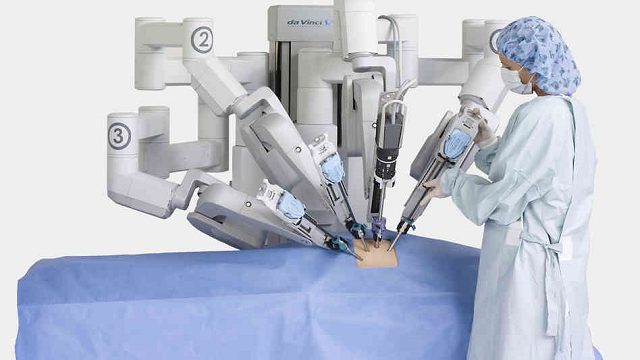
\includegraphics[width=1.1\pdfpagewidth]{da_vincy}%
%	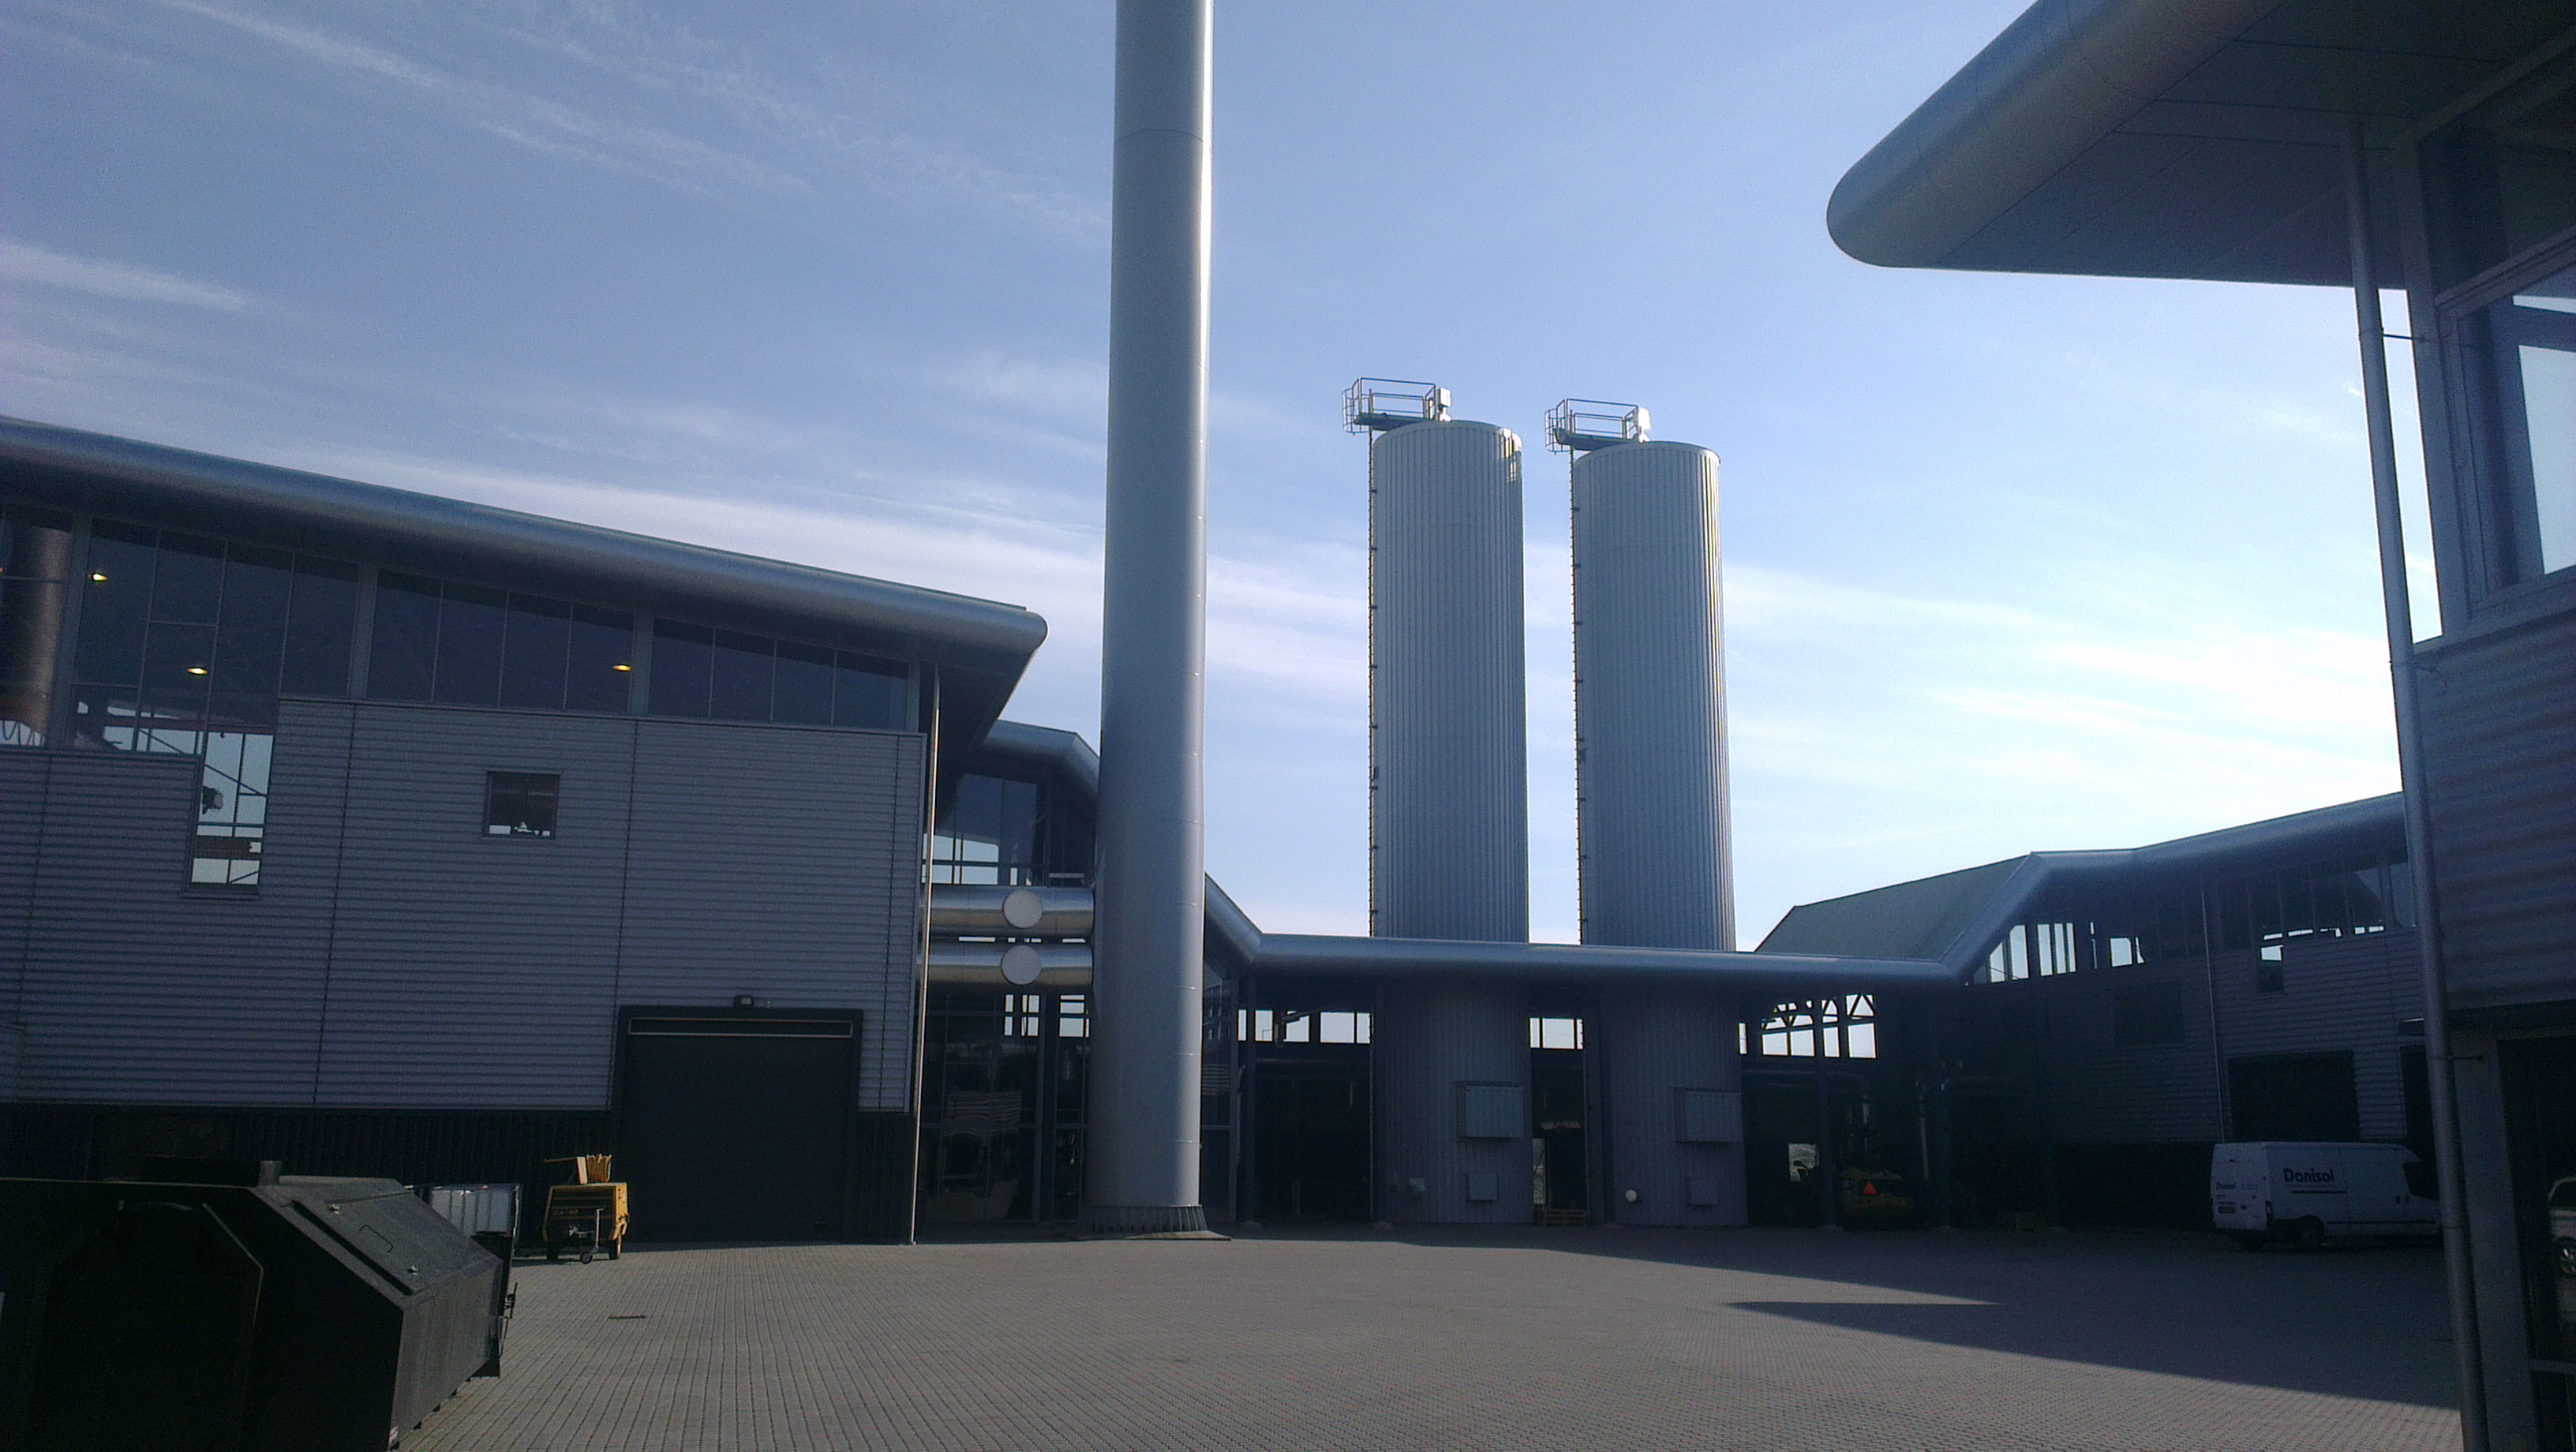
\includegraphics[width=0.45\pdfpagewidth]{formalia/2014-02-25 12.05.42.jpg}%	\caption{Virkningsgrad af den testede A/B hi-fi-forst�rker}
%\label{img_100wtest_linear}
\end{figure}
%\includepdf[scale=0.8,pages=1,pagecommand=\subsection{blub}]{testpdf}
%
\vspace{1cm}
\textsc{\Large \\
%Christian K�cks Lykkegaard \\
%s\\
%Economy track\\
%Elektronik \& IT\\
%Nordic Centre\\
%Fudan University\\
%September 27th 2012 \\
\textbf{School of Information and Communication Technology} \\
{\color{white}{..}}\\
Electronics \& IT\\
%s\\
Control and Automation \\
Final Thesis - CA4 Gr. 1032 \\
%Elektronik \& IT\\
Aalborg University\\
May 27$^\text{th}$ 2015\\
}\\
\end{titlepage}

\newpage
%\fchapter{}
\thispagestyle{empty}
%\begin{titlepage}
\vfil\null
\begin{center}
\bigskip \bigskip \bigskip
\vspace{1.0in}
\large
\bigskip \bigskip
\end{center} 
\normalsize
\vfil\null
\clearemptydoublepage
%\end{titlepage}

\thispagestyle{empty}
\begin{titlepage}


{\samepage 

\parbox{0.9\textwidth}{  
\raisebox{-15mm}{
\includegraphics[height=3.5cm]{AAU_LOGO_RGB_UK.png}}
\hfill{\footnotesize\noindent
\begin{tabular}{l}
            \textbf{School of Information and}\\
            \textbf{Communication Technology} \\
            Fredrik Bajers Vej 7 \\
            9220 Aalborg �st	\\
            Phone 99 40 86 00\\
            Fax 99 40 98 40\\
            http://www.es.aau.dk
\end{tabular}}}
\vspace{5mm}

    
\begin{tabular}{cc}
\parbox{7cm}{   
        {\bf Title:} Da Vinci Surgical Robot Automation \\        
        {\bf Master Thesis:} Control \& Automation\\              
        {\bf Project period:} Feb. $2^\text{nd} -$ June 3$^\text{rd}$ 2015\\
        {\bf Project group:} CA 15gr1032\\
        {\bf Participants:}\\
        \vspace{5mm}

\begin{minipage}[b]{0.7\linewidth}               	
     \underline{\phantom{JAERJAERJAERJAERoglidtmeretekst}}\\
      Britt Louise Jakobsen 
      
      \vspace{3mm}
	  
\includegraphics[width=0.52\textwidth]{IMG_3568_square.jpg}
\end{minipage}
  
\begin{minipage}[b]{0.7\linewidth}
   \vspace{10mm}
    \underline{\phantom{JAERJAERJAERJAERoglidtmeretekst}}\\
     Christian K{\o}cks Lykkegaard 

	\vspace{3mm}
	\includegraphics[width=0.52\textwidth]{IMG_3380.pdf}
\end{minipage}

\vspace{6mm}			
          
{\bf Supervisors:} \\
Prof. Rafa\l{} Wi\'{s}niewski\\
%Postdoc. Kasper Vinther\\
Ph.D. Tobias Leth\\
Assist. Prof. Christoffer Sloth\\
Postdoc. Karl Damkj�r Hansen\\  
               
        
{\bf Existing copies:} 5\\
{\bf Report:} \pageref{totalpage} pages \\
{\bf Appendix:} \pagedifference{appendixbegin}{appendixend} pages \\
\textbf{Attached:} 1 CD \\\\

\vfill } &
      
\parbox{7cm}{
\vspace{2mm}
\hfill 
\begin{tabular}{l}
      {\bf Abstract:}\bigskip \\
      \fbox{
      \parbox{7cm}{\bigskip
            {\vfill{\small In the course of the last few decades, robotic sur\-gery has become the  preferred type of operation within certain types of surgery, allowing the surgeon to perform precision procedures causing the patient a minimal amount of scarring while maintaining a exceptional overview of the operation site for the surgeon.


Advances are made within automation in the control of the robotic tools, providing the surgeon with more freedom and higher precision when performing operations. This thesis contributes to this advancement  through the use of barrier certificates with which safety of the automated control system can be guaranteed.


Control systems are developed for a number of use cases within robotic surgery for which safety  is certified through the construction of a barrier enclosing areas termed unsafe thus guaranteeing that the robotic tool will never cross this barrier. Two different approaches are taken: design of safety controllers based on manually constructed control barrier functions, and analytic verification of system safety using a software tool to construct the certificates.


The controllers are implemented on a first generation da Vinci surgical robot, and safety is verified for the developed control systems thus demonstrating the applicability of the theory of barrier certificates.


 \bigskip}}
      }\hspace{0.2em}}
\end{tabular}}

\end{tabular}

\vspace{-3mm}
\hspace{2mm}
\parbox{18cm}{
\noindent\footnotesize\textit{
\begin{flushleft} 
	The content of this report is freely available, but publication (with source reference) may only take place by agreement with the authors.	
\end{flushleft}}}
    
}
\end{titlepage}
\newpage
%\fchapter{}
\thispagestyle{empty}
%\begin{titlepage}
\vfil\null
\begin{center}
\bigskip \bigskip \bigskip
\vspace{1.0in}
\large
\bigskip \bigskip
\end{center} 
\normalsize
\vfil\null
\clearemptydoublepage
%\end{titlepage}

\setcounter{page}{1}
\renewcommand{\thepage}{\Roman{page}}

%\newgeometry{left=4.5cm,top=-0.5cm,bottom=2cm,textheight=28cm,includefoot,textwidth=16cm}
\chapter*{Preface}
\vspace*{-2mm}
This report documents the development process of a safe controller for automation of a surgical robot arm with patient safety guaranteed through barrier certificates. %, preventing the robot tool from entering predefined unsafe regions. 
The access to robot measurement data and opportunity to implement a controller heavily benefits from the previous work carried out on the da Vinci surgical robot in the Control Laboratory at Aalborg University.
The project is rated at 30 ECTS-points, and the work is conducted by the 4$^\text{th}$ semester group 1032 within the graduate program in Control and Automation at Aalborg University during the spring of 2015.


%The target group is supervisors, students and other interested parties at the School of Information and Communication Technology at the The Faculty of Engineering and Science.

\vspace*{-2mm}
\section*{Reading Guide}
\vspace*{-2mm}
The primary focus of this report is to design a controller and a barrier certificate, the certificate guaranteeing the safe control of a surgical robot, as an approach to draw closer to the possibility of implementing automated control tasks by surgical robots. 
%Controllers and certificates are designed for static as well as dynamic boundaries of unsafe regions, such as e.g. a beating heart.
After an introduction into surgical robotics and the definition of barrier certificates, two approaches to the design problem are described:
\vspace*{-3mm}
\begin{itemize}
\itemsep-1.4mm
\item Explicit approach: A barrier certificate is constructed and a safe controller is designed according to the method described in \citep{bib:org_control}.
\item Analytic approach: A controller is designed, criteria are constructed for a barrier certificate and  safety is verified by use of Putinar's Positivstellensatz.
%\item \autoref{part:closure} Discussion \textcolor{red}{REWRITE!!!}
\end{itemize}
\vspace*{-2mm}

Symbols, acronyms and a glossary are presented in the nomenclature before the main report.
A variant of the Harvard referencing is used for citations, with the author and publication year of the source given in square brackets, e.g. [Lasserre 78], and sources listed in the bibliography at the end of the main report. % contains all references used in the report. Books are indicated with author, title, publisher, year and ISBN. Web pages are indicated with author, title and year.
%Chapters in the main report are numerally numbered while appendices are alphabetically numbered.
A comprehensive appendix is included after the bibliography, containing introductions to the used software, detailed derivations, measurement logs and source code.
A digital copy of this report along with cited references, source code and simulation results can be found on the enclosed CD.

\vspace*{-2mm}
\section*{Acknowledgements}
\vspace*{-2mm}
The authors wish to thank Assistant Engineer Simon Jensen for a thorough introduction to the custom made AAU da Vinci hardware and design of a dynamic heart phantom platform; Ph.D. Tobias Leth for guidance in reference frame construction for robot kinematics;  Post Doc. Karl Damkj\ae r Hansen for an introduction to the AAU da Vinci robot operative system and help in implementing inverse kinematics; and Assistant Professor Christoffer Sloth for help and guidance with the theory behind barrier certificates and the use of SOSTOOLS.

Last but not least, it is desired to thank chief surgeon Johan Poulsen, robot assistant nurse Jane Petersson and surgeon Grazvydas Tuckus for sharing their insights in the use of surgical robotics and allowing the authors to attend a robotic surgery at Aalborg University Hospital.

%It is the wish of the authors to express a special appreciation to..

%\restoregeometry % efter denne side bruges de indstillinger der er sat i preamble
\newpage
%\fchapter{}
\thispagestyle{empty}
%\begin{titlepage}
\vfil\null
\begin{center}
\bigskip \bigskip \bigskip
\vspace{1.0in}
\large
\bigskip \bigskip
\end{center} 
\normalsize
\vfil\null
\clearemptydoublepage
%\end{titlepage}

\setlength\parskip{0ex}
\tableofcontents
\setlength\parskip{1ex}

%\nomenclature{$a_z$}{Acceleration in z direction\nomunit{[m/s$^2$]}}
\nomenclature{CO$_2$}{Carbon Dioxide}
\nomenclature{CHP}{Combined Heat and Power}
\nomenclature{DONG}{Danish Oil and Natural Gas}
\nomenclature{GEUS}{De Nationale Geologiske Unders\o gelser for Danmark og Gr\o nland (The National Geological Research for Denmark and Greenland)}
\nomenclature{BoP}{Balance of Payments}
\nomenclature{DFG}{Dansk Fjernvarmes Geotermiselskab (Danish District Heating Geothermal Corporation)}
\nomenclature{$Q_C$}{Heat-transfer rate: Condenser\nomunit{[$\text{kJ/s},  \text{kW}$]}}
\nomenclature{$Q_E$}{Heat-transfer rate: Evaporator\nomunit{[$\text{kJ/s},  \text{kW}$]}}
\nomenclature{$Q_K$}{Heat-transfer rate: Kettle HEX \nomunit{[$\text{kJ/s},  \text{kW}$]}}
\nomenclature{$Q_\text{SO}$}{Heat-transfer\,rate:\,Solution HEX\nomunit{[$\text{kJ/s} ,  \text{kW}$]}}
\nomenclature{$Q_\text{Geo}$}{Heat-transfer\,rate:\,Geoth.\,HEX \nomunit{[$\text{kJ/s},\text{kW}$]}}
\nomenclature{$\bar{Q}_C$}{Heat emitted: Condenser\nomunit{[kJ]}}
\nomenclature{$\bar{Q}_E$}{Heat absorbed: Evaporator\nomunit{[kJ]}}
\nomenclature{$W_\text{Comp}$}{Input work: Compressor\nomunit{[$\text{kJ/s} = \text{kW}$]}}
\nomenclature{ARS}{Absorption-Refrigeration System}
\nomenclature{$T_H$}{High temperature medium\nomunit{[$^{\circ}$C]}}
\nomenclature{$T_L$}{Low temperature medium\nomunit{[$^{\circ}$C]}}
\nomenclature{LiBr}{Lithium Bromide}
\nomenclature{SLT}{Second Law of Thermodynamics}
\nomenclature{SP}{Solution Pump}
\nomenclature{FLT}{First Law of Thermodynamics}
\nomenclature{$\text{HEX}_{\text{CW}}$}{Heat Exchanger - Cooling Water}
\nomenclature{$\text{HEX}_{\text{SO}}$}{Heat Exchanger - Solution}
\nomenclature{$\text{HEX}_{\text{K}}$}{Heat Exchanger - Kettle}
\nomenclature{$\text{HEX}_{\text{G}}$}{Heat Exchanger - Geothermal}
\nomenclature{$Q_A$}{Heat-transfer rate: Absorber\nomunit{[$\text{kJ/s}, \text{kW}$]}}
\nomenclature{$Q_G$}{Heat-transfer rate: Generator\nomunit{[$\text{kJ/s} , \text{kW}$]}}
\nomenclature{$\bar{Q}_A$}{Heat emitted: Absorber\nomunit{[$\text{kJ/s} ,  \text{kW}$]}}
\nomenclature{$\bar{Q}_G$}{Heat absorbed: Generator\nomunit{[$\text{kJ/s} , \text{kW}$]}}
%\nomenclature{Enthalpy}{Heat energy per unit mass\nomunit{[kJ/kg]}}
%\nomenclature{$Q_H$}{Heat emitted by Condenser\nomunit{[J]}}
%\nomenclature{$Q_L$}{Heat absorbed by Evaporator\nomunit{[J]}}
\nomenclature{$\bar{W}$}{Amount of work\nomunit{[kJ]}}
\nomenclature{$\text{COP}_\text{HP}$}{Coefficient of performance heat pump\nomunit{[$\cdot$]}}
\nomenclature{$\text{COP}_\text{R}$}{Coefficient of performance refrigerator\nomunit{[$\cdot$]}}
%\nomenclature{$m_3$}{Mass flow into Generator (liquid)\nomunit{[kg/s]}}
%\nomenclature{$m_{4}$}{Mass flow out of Generator (liquid)\nomunit{[kg/s]}}
%\nomenclature{$m_{7}$}{Mass flow out of Generator (vapor)\nomunit{[kg/s]}}
\nomenclature{$m_{n}$}{Mass flow at boundary $n$ \nomunit{[kg/s]}}
%\nomenclature{$h_{3}$}{Enthalpy into Generator (liquid)\nomunit{[kJ/kg]}}
%\nomenclature{$h_{4}$}{Enthalpy out of Generator (vapor)\nomunit{[kJ/kg]}}
%\nomenclature{$h_{7}$}{Enthalpy out of Generator (liquid)\nomunit{[kJ/kg]}}
\nomenclature{$h_{n}$}{Enthalpy at boundary $n$ \nomunit{[kJ/kg]}}
%\nomenclature{$p_{3}$}{Pressure into Generator (liquid)\nomunit{[Pa]}}
%\nomenclature{$p_{4}$}{Pressure out of Generator (liquid)\nomunit{[Pa]}}
%\nomenclature{$p_{7}$}{Pressure out of Generator (vapor)\nomunit{[Pa]}}
\nomenclature{$p_{n}$}{Pressure at boundary $n$ \nomunit{[Pa]}}
\nomenclature{$x_v$}{Vapor fraction\nomunit{[$\cdot$]}}
\nomenclature{$x$}{LiBr concentration\nomunit{[$\cdot$]}}
\nomenclature{$\text{EV}_1$}{Expansion Valve - Water Side}
\nomenclature{$\text{EV}_2$}{Expansion Valve - Solution Side}
\nomenclature{$\eta_\text{SHX}$}{Solution Heat Exchanger efficiency \nomunit{[$\cdot$]}}
\nomenclature{$\Delta T_{lm}$}{Log mean temperature difference\nomunit{[$^{\circ}$C]}}
\nomenclature{$U$}{Overall\,heat\,transfer\,coefficient\nomunit{[W/m$^2\, ^\circ$C]}}
\nomenclature{$A$}{Area\nomunit{[m$^2$]}}
\nomenclature{$W_\text{SO,P}$}{Input work: Solution Pump\nomunit{[$\text{kJ/s} = \text{kW}$]}}
\nomenclature{P-h}{Pressure-enthalpy}
\nomenclature{OD}{Valve Opening Degree}
\nomenclature{$\rho_\text{EV1,L}$}{Water density EV$_1$\nomunit{[kg/m$^3$]}}
\nomenclature{$\rho_\text{EV2,L}$}{Solution density EV$_2$ \nomunit{[kg/m$^3$]}}
\nomenclature{$C_{v}$}{Valve orifice constant  \nomunit{[1/(kg\,m)]}}
\nomenclature{SISO}{Single Input Single Output}
\nomenclature{MIMO}{Multiple Inputs Multiple Outputs}
\nomenclature{MPC}{Model Predictive Control}
\nomenclature{LQR}{Linear Quadratic Regulator}
\nomenclature{$c_\text{online}$}{Online computational time \nomunit{[s]}}
\nomenclature{LMMSEE}{Linear Minimum Mean Square Error Estimate}
\nomenclature{$L$}{Level \nomunit{[m]}}
\nomenclature{I/O}{Input/Output}
\nomenclature{SP}{Solution Pump}
\nomenclature{PC}{Pressure Control}
\nomenclature{PS}{Pressure Sensor}
\nomenclature{XC}{LiBr-concentration Control}
\nomenclature{XS}{LiBr-concentration Sensor}
\nomenclature{LC}{Level Control}
\nomenclature{LS}{Level Sensor}
\nomenclature{$L_E$}{Evaporator liquid level \nomunit{[m]}}
\nomenclature{$L_C$}{Condenser liquid level \nomunit{[m]}}
\nomenclature{$L_G$}{Generator liquid level \nomunit{[m]}}
\nomenclature{HEM}{Homogeneous Equilibrium Model}
\nomenclature{$V_\text{A,tot}$}{Total Absorber volume \nomunit{[m$^3$]}}
\nomenclature{$V_\text{A,L}$}{Volume of liquid part in Absorber \nomunit{[m$^3$]}}
\nomenclature{$V_\text{A,V}$}{Volume of vapor part in Absorber \nomunit{[m$^3$]}}
\nomenclature{$\rho_\text{A,L}$}{Absorber liquid density \nomunit{[kg/m$^3$]}}
\nomenclature{$\rho_\text{A,V}$}{Absorber vapor density \nomunit{[kg/m$^3$]}}
\nomenclature{$x_A$}{Absorber liquid LiBr/H$_2$O fraction \nomunit{[$\cdot$]}}
\nomenclature{$h_\text{A,L}$}{Absorber liquid specific enthalpy \nomunit{[kJ/kg]}}
\nomenclature{$h_\text{A,V}$}{Absorber vapor specific enthalpy \nomunit{[kJ/kg]}}
\nomenclature{$p_\text{A,V}$}{Absorber vapor pressure \nomunit{[Pa]}}
\nomenclature{$p_\text{A,L}$}{Absorber liquid pressure \nomunit{[Pa]}}
\nomenclature{$p_\text{A}$}{Absorber pressure \nomunit{[Pa]}}
\nomenclature{$T_\text{A,L}$}{Absorber liquid temperature \nomunit{[$^\circ$C]}}
\nomenclature{$T_\text{A,V}$}{Absorber vapor temperature \nomunit{[$^\circ$C]}}
\nomenclature{$M_\text{A,tot}$}{Absorber total mass \nomunit{[kg]}}
\nomenclature{$M_\text{A,L}$}{Absorber liquid mass \nomunit{[kg]}}
\nomenclature{$M_\text{A,V}$}{Absorber vapor mass \nomunit{[kg]}}
\nomenclature{$V_\text{G,tot}$}{Total Generator volume \nomunit{[m$^3$]}}
\nomenclature{$V_\text{G,L}$}{Volume of liquid part in Generator \nomunit{[m$^3$]}}
\nomenclature{$V_\text{G,V}$}{Volume of vapor part in Generator \nomunit{[m$^3$]}}
\nomenclature{$\rho_\text{G,L}$}{Generator liquid density \nomunit{[kg/m$^3$]}}
\nomenclature{$\rho_\text{G,V}$}{Generator vapor density \nomunit{[kg/m$^3$]}}
\nomenclature{$x_G$}{Generator liquid LiBr/H$_2$O fraction \nomunit{[$\cdot$]}}
\nomenclature{$h_\text{G,L}$}{Generator liquid specific enthalpy \nomunit{[kJ/kg]}}
\nomenclature{$h_\text{G,V}$}{Generator vapor specific enthalpy \nomunit{[kJ/kg]}}
\nomenclature{$p_\text{G,V}$}{Generator vapor pressure \nomunit{[Pa]}}
\nomenclature{$p_\text{G,L}$}{Generator liquid pressure \nomunit{[Pa]}}
\nomenclature{$p_\text{G}$}{Generator pressure \nomunit{[Pa]}}
\nomenclature{$T_\text{G,L}$}{Generator liquid temperature \nomunit{[$^\circ$C]}}
\nomenclature{$T_\text{G,V}$}{Generator vapor temperature \nomunit{[$^\circ$C]}}
\nomenclature{$M_\text{G,tot}$}{Generator total mass \nomunit{[kg]}}
\nomenclature{$M_\text{G,L}$}{Generator liquid mass \nomunit{[kg]}}
\nomenclature{$M_\text{G,V}$}{Generator vapor mass \nomunit{[kg]}}
\nomenclature{$V_\text{E,tot}$}{Total Evaporator volume \nomunit{[m$^3$]}}
\nomenclature{$V_\text{E,L}$}{Volume of liquid part in Evaporator \nomunit{[m$^3$]}}
\nomenclature{$V_\text{E,V}$}{Volume of vapor part in Evaporator \nomunit{[m$^3$]}}
\nomenclature{$\rho_\text{E,L}$}{Evaporator liquid density \nomunit{[kg/m$^3$]}}
\nomenclature{$\rho_\text{E,V}$}{Evaporator vapor density \nomunit{[kg/m$^3$]}}
\nomenclature{$h_\text{E,L}$}{Evaporator liquid specific enthalpy\nomunit{[kJ/kg]}}
\nomenclature{$h_\text{E,V}$}{Evaporator vapor specific enthalpy \nomunit{[kJ/kg]}}
\nomenclature{$p_\text{E,V}$}{Evaporator vapor pressure \nomunit{[Pa]}}
\nomenclature{$p_\text{E,L}$}{Evaporator liquid pressure \nomunit{[Pa]}}
\nomenclature{$p_\text{E}$}{Evaporator pressure \nomunit{[Pa]}}
\nomenclature{$T_\text{E,L}$}{Evaporator liquid temperature \nomunit{[$^\circ$C]}}
\nomenclature{$T_\text{E,V}$}{Evaporator vapor temperature \nomunit{[$^\circ$C]}}
\nomenclature{$M_\text{E,tot}$}{Evaporator total mass \nomunit{[kg]}}
\nomenclature{$M_\text{E,L}$}{Evaporator liquid mass \nomunit{[kg]}}
\nomenclature{$M_\text{E,V}$}{Evaporator vapor mass \nomunit{[kg]}}
\nomenclature{$V_\text{C,tot}$}{Total Condenser volume \nomunit{[m$^3$]}}
\nomenclature{$V_\text{C,L}$}{Volume of liquid part in Condenser \nomunit{[m$^3$]}}
\nomenclature{$V_\text{C,V}$}{Volume of vapor part in Condenser \nomunit{[m$^3$]}}
\nomenclature{$\rho_\text{C,L}$}{Condenser liquid density \nomunit{[kg/m$^3$]}}
\nomenclature{$\rho_\text{C,V}$}{Condenser vapor density \nomunit{[kg/m$^3$]}}
\nomenclature{$h_\text{C,L}$}{Condenser liquid specific enthalpy \nomunit{[kJ/kg]}}
\nomenclature{$h_\text{C,V}$}{Condenservapor specific enthalpy \nomunit{[kJ/kg]}}
\nomenclature{$p_\text{C,V}$}{Condenser vapor pressure \nomunit{[Pa]}}
\nomenclature{$p_\text{C,L}$}{Condenser liquid pressure \nomunit{[Pa]}}
\nomenclature{$p_\text{C}$}{Condenser pressure \nomunit{[Pa]}}
\nomenclature{$T_\text{C,L}$}{Condenser liquid temperature \nomunit{[$^\circ$C]}}
\nomenclature{$T_\text{C,V}$}{Condenser vapor temperature \nomunit{[$^\circ$C]}}
\nomenclature{$M_\text{C,tot}$}{Condenser total mass \nomunit{[kg]}}
\nomenclature{$M_\text{C,L}$}{Condenser liquid mass \nomunit{[kg]}}
\nomenclature{$M_\text{C,V}$}{Condenser vapor mass \nomunit{[kg]}}
\nomenclature{$V_P$}{Total volume of the pipe \nomunit{[m$^3$]}}
\nomenclature{$\rho_P$}{Density of the water in the pipe \nomunit{[kg/m$^3$]}}
\nomenclature{$c_P$ }{Specific heat of pipe liquid \nomunit{[kJ/(kg$\cdot^ \circ$C)]}}
\nomenclature{$T_\text{EX}$}{Temperature from the external model \nomunit{[$^\circ$C]}}
\nomenclature{$T_P$}{Temperature within the pipe \nomunit{[$^\circ$C]}}
\nomenclature{$\Delta T_{lm,P}$}{Pipe and the external model log mean temperature difference \nomunit{[$^\circ$C]}}
\nomenclature{$A_P$}{Pipe heat transferring related areal \nomunit{[$\text{m}^2$]}}
\nomenclature{$p_P$}{Pressure within the pipe \nomunit{[Pa]}}
\nomenclature{$c_\text{SO,P}$}{SP characteristics constant  \nomunit{[Pa/(m$^3$kg)] }}
\nomenclature{$\eta_\text{SO,P}$}{Solution pump efficiency \nomunit{[$\cdot$] }}
\nomenclature{SP}{Solution Pump}
\nomenclature{PI}{Proportional-Integral}
\nomenclature{PRBS}{Pseudo Random Binary Sequence}
\nomenclature{PDF}{Probability Density Function}
\nomenclature{FFT}{Fast Fourier Transform}
\nomenclature{$\mathbb{C}$}{Controllability matrix }
\nomenclature{$\mathbb{O}$}{Observability matrix }
\nomenclature{$T_s$}{Sampling time \nomunit{[s]}}
\nomenclature{$f_s$}{Sampling frequency \nomunit{[Hz]}}
\nomenclature{$N$}{MPC - horizon length}
\nomenclature{$y_\text{ref}$}{Output reference}
\nomenclature{$Q$}{MPC - weight on output error}
\nomenclature{$$R$$}{MPC\,-\,weight on change in control signal}
\nomenclature{TITO}{Two Inputs Two Outputs}
\nomenclature{$\text{COP}_\text{sim}$}{Coefficient of performance heat pump for simulation\nomunit{[$\cdot$]}}
\nomenclature{$\text{COP}_\text{lin}$}{Coefficient of performance heat pump linearised \nomunit{[$\cdot$]}}
\nomenclature{$m_C$}{Condenser district water mass flow\nomunit{[kg/s]}}
\nomenclature{$m_A$}{Absorber district water mass flow\nomunit{[kg/s]}}
\nomenclature{$m_E$}{Evaporator district mass water flow\nomunit{[kg/s]}}
\nomenclature{$m_G$}{Generator woodchip burner water mass flow\nomunit{[kg/s]}}
\nomenclature{$C_W$}{water Specific Heat Capacity\nomunit{[(J/Kg)$^\circ$C]}}
\nomenclature{$A_\text{s,c}$}{System matrix continuous time}
\nomenclature{$B_\text{s,c}$}{System actuator matrix continuous time}
\nomenclature{$C_\text{s,c}$}{System sensor matrix continuous time}
\nomenclature{$D_\text{s,c}$}{System feed-forward matrix continuous time}
\nomenclature{$A_\text{s,dt}$}{System matrix discrete time}
\nomenclature{$B_\text{s,dt}$}{System actuator matrix discrete time}
\nomenclature{$C_\text{s,dt}$}{System sensor matrix discrete time}
\nomenclature{$D_\text{s,dt}$}{System feed-forward matrix discrete time}
\nomenclature{$A_\text{d}$}{Disturbance system matrix}
\nomenclature{$B_\text{d}$}{Disturbance actuator matrix}
\nomenclature{$C_\text{d}$}{Disturbance sensor matrix}
\nomenclature{$D_\text{d}$}{Disturbance feed-forward matrix}
\nomenclature{$A_\text{aug}$}{Augmented system matrix}
\nomenclature{$B_\text{aug}$}{Augmented actuator matrix}
\nomenclature{$C_\text{aug}$}{Augmented sensor matrix discrete}
\nomenclature{$D_\text{aug}$}{Augmented feed-forward matrix}
\nomenclature{$L_\text{aug}$}{Augmented observer gain}
\nomenclature{$L_1$}{System model observer gain}
\nomenclature{$L_2$}{Disturbance model observer gain}
\nomenclature{$\xi$}{Improvement of COP \nomunit{[\%]}}

\printnomenclature \label{chap:acronym}

\printglossary[type=symbols,style=long4col]

\section*{General Nomenclature Remarks}
\vspace{0.1cm}
\begin{itemize}
\item The notation is..
\item Well..
\end{itemize}

\cleardoublepage
\setcounter{page}{1}
\renewcommand{\thepage}{\arabic{page}}

\chapter{Introduction}\label{chap:intro}
In minimally invasive surgery (MIS), as opposed to traditional open surgery, only small incisions are made in the patient's abdomen or pelvis in order to gain access to the area under surgery, hence causing less trauma beyond this confined area. This in general provides the patient with quicker recovery, shorter hospital stay and less scarring.
One type of MIS is laparoscopy, invented in the beginning of the 20th century \citep{bib:laparoscopy}, where thin metal telescopes (laparoscopes) with specialized surgical tools attached are inserted into the patient through trocars, allowing the surgeon to maneuver the tools in the inflated abdomen guided by visual feedback from a flexible miniature camera (endoscope) inserted alongside the surgical tools \citep{bib:fascrs}.
In the 1980s robotic laparoscopic surgery was introduced as a master-slave system, where the surgeon controls a robot arm holding the surgical tools from a master console, instead of manipulating the instruments manually.

\section{Highlights in the Development of Surgical Robotics}
While the idea of roboticized telemedicine dates back to 1925 \citep{bib:telemed_predict}, the development of telesurgery was founded by NASA (National Aeronautics and Space Administration) in the 1970s \citep{bib:telesurg_history} combining research within virtual reality, robotics and medicine \citep{bib:brown_univ}, and the first robotic surgery procedure was accomplished in 1985 \citep{bib:telesurg_history}, followed by the first laparoscopic robotic surgical procedure in 1987 \citep{bib:brown_univ}.
The major research within telesurgery was funded by DARPA (Defence Advanced Research Project Administration, research administration under the U.S. Department of Defence) in the early 1990s, and two main teleoperation systems were developed from this research: da Vinci (from Intuitive Surgical) and Zeus (from Computer Motion) \citep{bib:telesurg_history}.

The first commercially available surgical robot ROBODOC (from Curexo) was introduced and performed the first robotic joint replacement surgery in 1992, and in 1994 the AESOP (from Computer Motion) was the first robotic system approved by the FDA (U.S. Food and Drug Administration) for general surgery \citep[p 74]{bib:telesurg_history,bib:surgical_book}.

In the early 1990s the U.S. Army developed MASH (Mobile Advanced Surgical Hospital) for loading and teleoperating wounded soldiers in vehicular operating rooms \citep{bib:brown_univ}, and in 1993 the idea for a robotic slave manipulator arm was conceived by Madhani after watching an episode of the tv-show M*A*S*H [SurgRob], and he created the Black Falcon during his work at MIT \citep{bib:black_falcon} later becoming he prototype of the da Vinci arms.

In 1996 the first tests were performed demonstrating the successful use of telementoring and telemanipulation of the endoscope by a surgeon placed several 100 m away from the operating room \citep{bib:telesurg_history}. 
In the late 1990s NASA and DARPA sponsored research within light-weight and deployable space surgical robotics for remote teleoperation, resulting in two main robotic systems: the Raven (from University of Washington) and M7 (from SRI International) [SurgRob].

In 1998 Zeus (from Computer Motion) was introduced and performed the first fully endoscopic robotic surgery and the initial beating-heart totally endoscopic coronary bypass procedure \citep{bib:brown_univ} and in 2000 da Vinci (from Intuitive Surgical) became the first robotic surgical system  to be approved by the FDA for general laparoscopic surgery \citep{bib:mddi}.

The first transatlantic telesurgical procedure, the Lindbergh Operation, was performed in 2001 by a team of French doctors in New York manipulating the arms of a Zeus robot to perform a gall bladder operation on a patient in Strasbourg \citep{bib:telesurg_history}. More research into remotely telementored and teleoperated robotic surgery was performed in the 2000s with the NEEMO (NASA Extreme Environment Mission Operations) projects in the Aquarius undersea lab in Florida, in 2003 with Zeus controlled from Ontario 2500 km away \citep[pp 75, 81]{bib:surgical_book} and in 2006 and 2007 with Raven and M7 controlled from Seattle \citep[pp 28, 82]{bib:surgical_book}. 

In 2005 DARPA launched the Trauma Pod program for developing an unmanned autonomous and semi-autonomous mobile military operation platform, funding research for e.g. SRI and for the Raven project. The goal of the first phase of the project was achieved in 2007 with the successful demonstration of a prototype trauma pod consisting of a da Vinci robot, a MASH stretcher and a custom nurse robot \citep[p 30]{bib:surgical_book}. The second phase aims at miniaturizing and integrating the systems \citep[p 31]{bib:surgical_book}, and in 2005 a demonstration was performed by roboticists, surgeons, aerospace engineers and networking experts in the desert placing the Raven patient manipulator and the controller console 100 m apart and relaying the communication link via a drone \citep{bib:docatadist}.

%In 2006 the first-ever demonstration of unmanned telesurgery with M7 [SurgRob]
%
%M7 performed the world's first automated ultrasound guided tumor biopsy in 2007 [SurgRob]
%
%2008 neuroArm was first used to remove a brain tumor [SurgRob]

NASA's first experiment in a zero gravity environment was performed with an acceleration compensated M7 in 2007 on a parabolic flight \citep[pp 29, 76, 85]{bib:surgical_book}, and in 2011 NASA sent the humanoid robot Robonaut 2 to ISS (International Space Station), and it has since been trained in telemedicine [SurgRob].







\section{State-of-the-Art in Surgical Robotics}
Most surgical robots used for telesurgery are master-slave systems which can be fully controlled by the surgeon \citep{bib:raven_debride}. The patient manipulator consists of 2-4 robotic arms, each having 6-7 degrees of freedom (DOF) \citep{bib:raven_debride} including the arm, wrist and the end-effector (the laparoscopic tool), one of the arms holding a stereo-vision endoscope. The end-effectors are positioned by high-precision motors and are able to reach spaces a human hand cannot \citep{bib:docatadist}.
Development is progressing within flexible end-effector tools \citep[p 74]{bib:surgical_book}, but even microrobots entering the body through natural orifices and controlled via electromagnetic fields or nanosensors and -actuators are being developed [SurgRob].

The 3D visual feedback from the endoscope is sent to the master console which can have eye-tracking for adaptive field of view and safety stop if the surgeon's gaze is not fixed at the operation site [SurgRob]. The control signals for the surgical instrument are generated with the controller joystick, which scales the surgeon's movements down to micro-movements \citep{bib:intuitive_monopoly} steerable through the (zoomed) 3D visual feedback. It also filters away tremor, and development is made within haptic feedback to the joystick \citep[p 89]{bib:surgical_book}, enhancing the surgeon's feel, enabling greater dexterity, accuracy and stability than a human hand.

In the first generations of surgical robotics the master and slave had to be in the same room (as is the case with da Vinci) \citep{bib:telesurg_history,bib:raven_debride,bib:surgical_book}. Experiments and development are made within minimizing and coping with delays for long-distance telesurgery and within miniaturization and robustness of the surgical robotic systems for use in harsh environments such as war and space, e.g. for da Vinci's potentially closest competitor, the open-source Raven.

Robotic surgical procedures are beginning to show superiority to conventional surgery for some procedures, but is still considerably more ecpensive \citep{bib:docatadist}. In some cases robotic procedures are faster than conventional surgeon procedures [SurgRob], but still in other it is much slower \citep{bib:raven_ii,bib:raven_debride}.
Autonomous procedures are still only implemented for entirely pre-planned motions of an operation, and depending on the type of operation not all subtasks in an operation are suited for autonomy \citep{bib:raven_debride,bib:raven_ii}.


\textcolor{red}{New generation: surgical care not only to soldiers but also to remote locations lacking specialized physicians. - better tactile feedback because the surgeon needs to feel the tissue and the difference in its stiffness}

Although the feasibility of conducting surgical interventions remotely has been demonstrated, there has not been market or clinical drivers strong enough to justify its implementation \citep[p 38]{bib:surgical_book}

\subsection{The da Vinci Surgical System}
Although several FDA approved robotic surgical systems exist, da Vinci is still the only commercially available system \citep{bib:docatadist,bib:intuitive_monopoly}. The first da Vinci prototype was developed at SRI under contract with the U.S. Army in the late 1980s [MDD], \citep{bib:brown_univ}, and in the early 1990s DARPA invested in the research \citep[p 74]{bib:surgical_book}. The the mid 1990s SRI licensed the manipulator design of Madhani along with many other patents, and in 1995 SRI founded Insuitive Surgical and the focus shifted from battlefield to commercial use in hospitals \citep{bib:intuitive_monopoly}.
In 1997 the first human trials were performed \citep{bib:intuitive_monopoly}, in 1999 the first market-ready da Vinci began tests [SurgRob] and the system was first approved by the FDA in 2000 \citep{bib:intuitive_monopoly,bib:brown_univ}. From 2000 until the merger in 2003 Intuitive Surgical and Computer Motion had a number of lengthy patent litigations \citep{bib:intuitive_monopoly,bib:telesurg_history}.

The da Vinci Surgical System still has the predominant market share with more than 3000 units installed worldwide due to being the first-mover in the field and due to their many patents \citep{bib:intuitive_monopoly}, and has only had one serious case of a patient dying after surgery (2002) [SurgRob].
The expiration of their patents in 2015 and 2016 \citep{bib:intuitive_monopoly} shows promise of many other robotic surgery systems entering the market, as both American, Canadian, European and not least Asian similar systems exist that are considerably cheaper than the da Vinci, and also more lightweight.

In 2013 Intuitive released the da Vinci Research Kit platform, built from mechanical components from first generation da Vinci (two arms and a surgeon console), open-source electronics and university-developed software \citep{bib:raven_observ}.

\subsection{The Raven Surgical Robot}
One potential challenger to da Vinci is the Raven \cite{bib:mddi}, an light-weight open-architecture 2-armed surgical robot \citep{bib:raven_debride,bib:raven_ii} originally developed by University of Washington funded by multiple U.S. government agencies including the Army and the Department of Defence (DoD) \citep[p 27]{bib:surgical_book}.
Raven-II is installed at 10 different universities in the U.S. and one in France \citep{bib:raven_ii}, sharing research innovations and using open-source software (including the ROS middleware) to create surgery subtasks \citep{bib:raven_debride}. 
As Intuitive Surgical's patents gradually expire the University of Washington is considering the possibility of spinning off the Raven into a start-up company \citep{bib:economist}.

The Raven robot is focused on remote telesurgery (with notable latency) in harsh conditions \citep{bib:docatadist}, and research at University of California has been made in teaching a computer model to autonomously mimic laparoscopic surgeons from recordings dynamic and kinematic data of their motions in a multi-state statistical Hidden Markov Model \citep{bib:economist}. 
The primary difficulty reported from controlling the Raven has been state estimation, necessary because of the uncertainty inherent in actuators and encoders connected to flexible elements via long cables \citep{bib:raven_debride} and the necessity of collision avoidance of the arms.



































\section{Focus of this Project}
Our focus:
safety
make forbidden areas where the robot cannot enter

ROS middleware layer as in Raven.
Prior work: designing planning and control algorithms for autonomous execution of several surgical subtasks (knot tying, suturing), advances in motion planning, control and perception: integrated task and motion planning ofhigh level task planning using state machines, and motion planning for low level planning algorithm  \citep{bib:raven_debride}
Raven-II inverse control process (not primarily to estimate the pose, in which case standard estimation methods like Kalman would be appropriate) is to calculate, give an desired true pose, the input pose to send the control sw to reach the desired true pose (detected pose with vision system assumed to be the true pose), estimate between measurements using updates from forward kinematics \citep{bib:raven_debride}.
da Vinci Research Kit: learning from demonstrations/by observation. Targets considered form convex regions spherical/linear. Patient Side Manipulators manipulates the instruments about a fixed point called the remote center of motion \citep{bib:raven_observ}.
DLR MIRo integrates torque sensing capabilities on the joint level, cosisting of actuation- position sensing- and torque sensing modules, can run in torque and impedance control mode. Virtual springs/potential fields are used to impose constraint forces preventing the robot from  entering predefined areas.


One should certainly take the risk of patient trauma when an automated surgery is conducted into account. This is seen in Therac-25. It is therefore a necessity to formally prove that the procedure is safe as seen in \citep{bib:safety}
\section{Technical Overview}
A simplified overview of the overall setup is provided in \autoref{fig:overview} as a block diagram. The setup is physically located at the department of Control and Automation at Aalborg University in the laboratory. The figure is structured with the highest abstraction layer at the top (i.e. the ROS (Robotic Operation System) - a software framework for robots [ROS artikkel]) environment which establish a wireless TCP/IP communication channel receiving all positions from the robot as feedback. It produces likewise positioning control signals to the NI (National Instruments) single board RIOs (Reconfigurable Input/Output) which handle all input/output communication with the user. The NI single board RIOs consist of a primary and a secondary board. The reason for having two RIO boards is solely the lack of input/outputs on one board.

The RIO boards direct the control signals to a cascaded controller taking in a velocity reference from the user and delivers a current control signal to the ESCON motor driver. The velocity and current controller are implemented in FPGA based hardware to ensure sufficient controller speed relative to the system \citep{bib:robot_paper}. The ESCON motor driver manage advanced processing and delivers essentially an appropriate PWM signal for the  actuators in form of seven maxon motors which represent the lowest abstraction layer located at the bottom of the figure.

The NI single board RIOs handle concurrently most safety precautions and enabling/disabling of the arm itself (see appendix ?? for location of the arm) through solenoids.
\begin{figure}[H]
	\center
	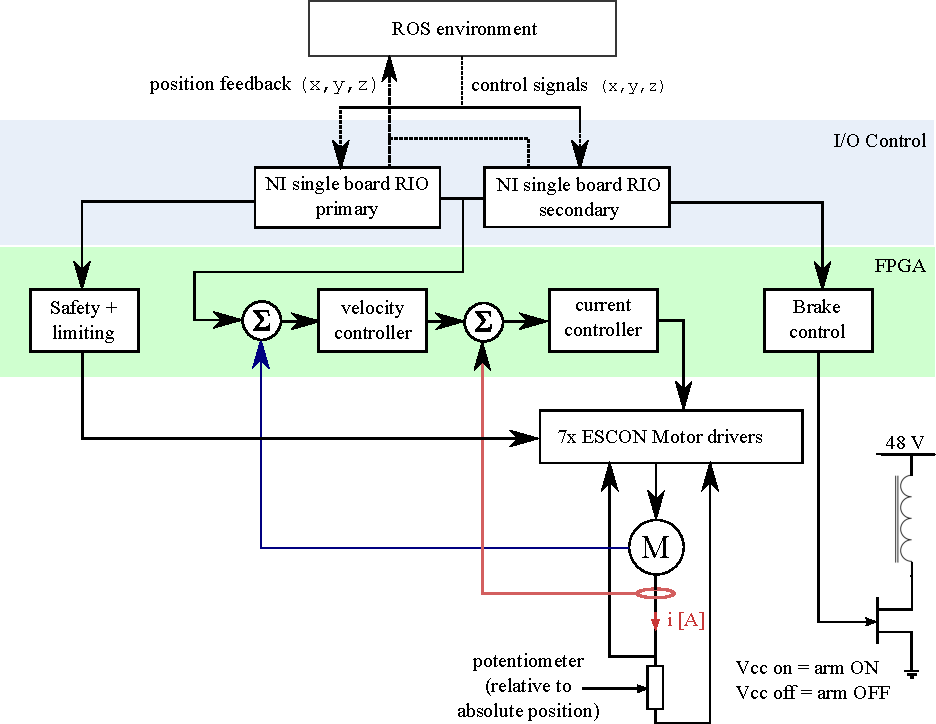
\includegraphics[width=0.95\textwidth]{overview.pdf}	\caption{This is a nice figure. Here illustrated for hand roll master.}
	\label{fig:overview}
\end{figure}
The focus of this thesis is the highest abstraction layer, i.e.the ROS environment. The purpose here primary constitute implementation of:
\begin{itemize}
\item Everything that require heavy processing \citep{bib:robot_paper}.
\item Non real-time processing or tasks with loose timing constraints \citep{bib:robot_paper}.
\end{itemize}
The above pool of stipulations will essentially and practically entail the follow main topics of this thesis:
\begin{itemize}
\item All user interaction
\item Positioning control loop
\item Path planning
\end{itemize}
bla-bla \gls{phi} \gls{gammacl}  \gls{dbar} \gls{T} \gls{B}
fsa
\gls{ROS}
\part{System Analysis}\label{part:part1}

\chapter{Basic Concepts}\label{basic_stuff}

\chapter{Interim Conclusion} \label{chap:interim_con}
%\vspace{-0.3cm}
An introduction to the concept of automated surgery with robotic manipulators is given in \autoref{chap:intro}. It founds the need for a way to guarantee safety in such operations. Thus, the initial task posed in \autoref{sec:project_overview} concerns two approached to the problem of ensuring safety for the da Vinci robotic manipulator, i.e.:
%\vspace{-0.3cm}
\begin{enumerate}
\item The design of a safe controller ensuring safety in real-time. 
\item The analysis of a controller, posing the question if it is safe. 
\end{enumerate}
%\vspace{-0.3cm}
The first bullet point is at this point investigated. The theory presented in \citep{bib:org_control} is adopted and described in \autoref{chap:cbf} which ensures that the barrier certificates outlined in \autoref{chap:barrier_cerificates} are obeyed, thereby allowing the development of safe controllers.

The theory is applied to specific use cases. First, a palpable example is conducted in \autoref{chap:cbf_1d_static} which ought to give experience with control barrier functions (CBFs) and the way the theory is applied. The outcome is not only a fully functional safe controller in one dimension, but also a valuable experience. As expected, when the system order increases, the difficulty in constructing valid CBF, is also increased. Though, with a system order $n=2$, it is indeed still possible. Primary because the states can be translated into physical meaningful quantities such as position and velocity. However, it is easy to imagine that as $n$ increases and the meaningful states vanish to abstract states, this approach will be as good as impossible.

The next step is taken in \autoref{chap:cbf_1d_dynamic} where the problem consist of ensuring safety for a beating heart, such that a virtual fixture can be ensured in a safe manner. The problem here differs from \autoref{chap:cbf_1d_static} because the CBF is dynamic. Though, again, a successful implementation is performed and a valid CBF can be found. The dimensions of the system is kept low which simplifies the task of finding a valid CBF. The lack of integral action is obvious in this chapter and with a more advanced/realistic model of the heart, the search for a valid CBF will be a highly non-trivial task. If not impossible.

The dimensions is yet again increased in \autoref{chap:cbf_3d_static}. A safe controller in the 3D euclidean space is developed with an associated valid CBF alongside. It is from here seen that the creativity and complexity increases yet a step. With a simplified model of the robotic manipulator, a successful analysis and implementation is performed. The result is as expected and indeed quite convincing, but it is also clear that to reach the end goal of a realistic model of the heart or other vital organs and of the robotic manipulator, the system order must be increased. Again, this implies serious challenges in the construction of a valid CBF.

%can be difficult to find a barrier certificate that is valid for a system, especially as the order of the system grows, as seen from the second order system

Accordingly, it is desirable to find a different approach to defining barrier certificates that is more efficient for higher order systems. Indeed, an efficient and straight forward approach may be difficult to derive, but the success criteria for a higher order system can more appropriate be defined as: \textit{If it is possible, it is better.} This is where the second bullet points become active.

The MATLAB toolbox SOSTOOLS can be used to perform a "controller analysis". This toolbox uses Sums of Squares optimization to solve problems, so it is necessary to cast the definition of the barrier certificate as an SOS program to use it for barrier certificate search. Hence the background to the SOS  formulation of the problem is presented in the upcoming chapter, after which the SOSTOOLS toolbox is introduced, and used for barrier certificate search.

This approach intends to solve the second bullet point, i.e. to find a way to analyse if the controller is safe, thereby giving it a "safe" or "not safe" verdict.

\chapter{Requirement Specification}\label{chap:reqspec}
A list of the requirements is probably necessary if things should remain beautiful.

\part{Controller Design}\label{part:part2}
\chapter{Control System Introduction}\label{chap:systemdesign}

\part{Discussion}\label{part:part3}
\chapter{Conclusion}\label{chap:conclusion}
This chapter will conclude on the results obtained throughout this thesis and put the solution and entire strategy into perspective in the discussion part.
\section*{Conclusion}
Safety aspects in robotic surgery and automated robotic surgery are found to be \textit{the} important factor, as analysed in \autoref{chap:intro}. Concurrently, it founds the basic framework in the long term goal of obtaining virtual fixtures. Consequently, a barrier certificate is stated in \autoref{chap:barrier_cerificates} which modifies and adapts the Lyapunov stability criteria to enable a way to define  safe and unsafe regions within the state-space. 

A theoretical controller is developed in \autoref{chap:cbf} based on control barrier functions which ensures that the  barrier certificate requirements presented in \autoref{chap:barrier_cerificates} are obeyed at all times. Thus, the control barrier function allows a way to ensure safety in real-time with astounding few calculations.

The control topology presented in \autoref{chap:cbf} is applied to three use cases which intend to commence a solution to the problem of guaranteeing safety in automated surgeries, i.e.:
\begin{itemize}
\item A concrete example of the use of control barrier functions is founded in \autoref{chap:cbf_1d_static}. It comprises the instrument slide movement. The system is modelled as both a first and second order system, thereby slowly increasing the complexity of the CBFs, such that necessary experience in the construction of CBFs can be gathered. The result is a successful controller guaranteeing safety by never entering predefined unsafe regions in one dimension for both a first and second order system approximation.
\item A safe regulator is designed to ensure system safety in relation to virtual fixtures in \autoref{chap:cbf_1d_dynamic}. A dynamic CBF is  constructed in accordance with the desire of virtual fixture and thus founds safety for operation on a beating heart. The result for this use case is that a safe distance between heart and robotic end effector can be set as desired.
\item Then safety considerations are extended to the 3D Euclidean space in \autoref{chap:cbf_3d_static} which implies additional implementation challenges such as a kinematic description (mapped and verified in \autoref{app:kinematic_model_robot}), forward kinematics and inverse kinematics. The construction of a CBF is taken to higher dimensions forming a barrier enclosing the interior of an ellipsoid, thus representing a heart or another vital organ fixed in space. The result is a valid CBF ensuring that the robot end effector is kept outside the ellipsoid at all time.
\end{itemize}
All three use cases are implemented in a simulation environment in MATLAB with convincing results, i.e. system safety is ensured by preventing the system state from entering specified unsafe regions. The controllers are furthermore implemented in C++ in the ROS (Robotic Operating System) framework. The ROS framework is founded in \autoref{app:ros} as a necessary condition to allow any implementation on the da Vinci robot. All development within ROS is tailored for this project and did not exist at project initiation. The implemented controllers comply with the expected outcome and do indeed behave as desired, i.e. ensuring safety by evading the predefined unsafe regions. Additionally, the implemented controllers are verified to require very little processing power making them ideal as real-time controllers.

The three use cases do, however, consist of simple models where the system order does not exceed 3. An important conclusion is drawn from the use cases, which already could be inferred from the one dimensional safe slide controller (developed in \autoref{chap:cbf_1d_static}) with system order 2. That is, for high order systems where the physical interpretation of the state vector is obscured, the construction of a valid CBF is a highly non-trivial task -- if not impossible. 

For this reason, the problem is turned upside down in \autoref{chap:putinar}, thus no restrictions are put forth in the controller development. Instead, the closed loop system is evaluated and the question is asked whether it complies with the barrier certificate requirement in \autoref{chap:barrier_cerificates}. The verdict is hereafter given as \textit{pass} or \textit{not pass}. For this purpose, \autoref{chap:putinar} presents the global SOS (Sum Of Squares) positivity characteristic and through Putinar's Positivstellensatz recast the barrier certificate formulation as a  problem of local positivity, thus allowing sets of unsafe and safe regions to be defined by unrestricted polynomials.

The strategy presented in \autoref{chap:putinar} is applied with the MATLAB toolbox SOSTOOLS in \autoref{chap:sostools} such that  barrier certificates can be searched for by automated means. Here, a framework is developed such that the toolbox takes a closed loop system description and a description of the safe and unsafe regions as inputs. The developed framework delivers an unambiguous certificate answering if the system is safe, thus constituting the \textit{pass} and \textit{not pass} verdict. The slide controller developed in \autoref{chap:cbf_3d_static} is accordingly taken as an example and the framework is verified with this example. Both the first and second order system approximation is analysed in the designed SOSTOOLS framework. It is, as expected, certified to be safe in almost the entire desired range.  These examples conclude and verify the use of the developed framework. The framework can easily handle other systems, as the task merely comprises other closed loop system descriptions as input in other dimensions with different safe and unsafe sets. This is a trivial task.

Hence, it can be concluded that the two initially desired strategies comprising the design and analysis of a safe controller are investigated and solved sufficiently to provide a "proof of concept" framework. This applies for both theory, simulation and implementation.


\section*{Discussion and Future Work}
The developed solution proves itself very efficient in both theory and simulation. However, the implementation aspect suffers from a number of issues which should be investigated in future work. This includes:
\begin{itemize}
\item Incorporate integral action in all controllers to eliminate steady state errors.
\item Increase the sampling rate from 100\,Hz to 2\,kHz which indeed is the long term goal. All controllers will draw benefits from this on the transition set $\mathcal{T}$. This may, however, introduce challenges as the allowed execution time (process time between every sample) is lowered to 0.5\,ms which is less than the actual execution time in \autoref{fig:3d_exe} for the safety controller in the 3D Euclidean space. Therefore, optimization must be performed in the implementation.
\item Improvement of the inverse kinematics solver as it occasionally chooses joint angles requiring multiple revolutions around the unit circle to obtain a position which could be reached with an angle less than $\pi$.
\end{itemize}
Additionally, the position controller already implemented on the FPGA (as seen in \autoref{fig:overview}), is left untouched. It may with removed to draw benefits from a more clear dynamics. This will require another system model, but may well be worth the trouble.

Furthermore, a consistently disregarded topic in this project is the use of trajectory planning. The controllers developed take only small steps as input. However, large step sizes have been given to the controllers in this project to demonstrate certain features, but obviously, it is desired to construct a trajectory planning layer taking the setpoints as input and breaking the path down into a sequence of adjacent points, thus ensuring that small step sizes are given to the controller.

Additionally, at no point  the orientation of the robot hand has been considered. Obviously, ensuring safety for the end effector is not sufficient as the heart or other vital organs can be penetrated or crushed by collision with the physical volume of the robotic tool other than the tip of the tool. This is an important topic in future work. Collision avoidance for the robotic parts themselves must also be studied when employing all four of the da Vinci arms in the setup, which is indeed the long term objective.

It is suggested for future use of the framework developed for barrier certificate search with SOSTOOLS to conduct the search in a more methodical manner by running the search like a Monte Carlo simulation, each time varying a parameter while keeping the others fixed. In this way the chance of determining a valid barrier function is maximized, thus indispensably invalidating system safety if no valid certificate can be found.

As explained by assistant nurse Jane Petersson in \autoref{sec:aau_doc}, there are veins, nerves and other organs which must not be cut during a surgery. It has been the aim to construct barrier certificates that can represent these parts of the body. However, it is clear that a realistic barrier certificate representing these parts is far away. Especially because they are time dependent and because, from time to time, the surgeon needs to move these parts to be able to operate in a certain area, thus reshaping these parts. Consequently, a very creative and adaptive barrier function is required and will as a necessary condition require robot vision (a continuous video stream analysis) such that these parts can be tracked. A way to resolve this complex problem of high dimensionality could be a combination of the design approach and analysis approach in the following way:
\vspace{-1.5mm}
\begin{enumerate}
	\itemsep-0.5mm
\item Search for a barrier certificate using the framework developed in \autoref{chap:sostools}.
\item Apply this barrier certificate as control barrier function in a similar way as done in \autoref{chap:cbf_1d_static}, \autoref{chap:cbf_1d_dynamic} and \autoref{chap:cbf_3d_static}.
\item Analyse the situation. Adjust the barrier certificate if necessary and describe the new closed loop system.
\item Take the new closed loop system as input to the framework developed in \autoref{chap:sostools} and start from 1 again.
\end{enumerate}
This iterative approach may along with the preceding listed bullet points get the robotic surgery industry one step closer to the end goal of guaranteed safe robotic surgery with the da Vinci robot,
which has been the sole application of the safety controllers derived throughout this project. However, it should take very little imagination to envisage that this way of constructing controllers has the potential to be used in many other industries where safety is critical or simply where regions are desirable to be left untouched.

\chapter{Perspective}\label{chap:perspektivering}
This will become a very nice and beautiful perspective.

\begingroup
\raggedright
\clearpage
\addcontentsline{toc}{chapter}{Literature}
\bibliography{bibtex/litteratur}
\endgroup
\label{sourceliste}

\newpage

\begin{appendices}
\appendix
%\renewcommand{\appendixname}{Appendices}
\renewcommand{\appendixname}{Appendix}
\renewcommand{\appendixtocname}{Appendix}

\chapter{My First Appendix}\label{app:vest}

\chapter{MATLAB Code}\label{app:source}

\chapter{Attached CD} \label{chap:cd}
\subsection*{Datasheets}
\subsection*{MATLAB Scripts}

\end{appendices}
\end{document}